\scanpage{70}
\mspage{69}
\mspage{28}
\margin{démonstration peu \unsure{naturelle}\ \unsure{\P}}
\margin{\figure{\begin{tikzpicture}[x=1cm,y=1cm]\draw (.2,0)--(0,0)--(0,-.8)--(.15,-.8);\draw[very thin] (-.8,-.7)..controls (-.9,-1.6) and (-.85,-2.7)..(-.85,-3.5);\end{tikzpicture}}}
Démonstration. La première assertion veut naturellement dire que pour $S'\xrightarrow{u}S$ arbitraire, le morphisme
\diagram{\[
\begin{tikzcd}
{u'}^*(R^qj_*)g^*F\arrow[r]&(R^qj'_*){g'}^*u^*F
\end{tikzcd}
\]}
est bijectif dans les situations envisagées, où $u'=u\times_S X$, et la dernière assertion équivaut à la première pour les faisceaux abeliens (IV4.5.).

Pour $q=0$, on a (3.2) des isomorphismes
\diagram{\[
\begin{tikzcd}[row sep=large]
{u'}^*f^*F\arrow[r,"\sim"]\arrow[d,phantom,"{\rotatebox{90}{$\simeq$}}" description]&{u'}^*j_*g^*F\\
{f'}^*u^*F\arrow[r,"\sim"]&j'_*{g'}^*u^*F
\end{tikzcd}
\]}
d'où le résultat.

\margin{\figure{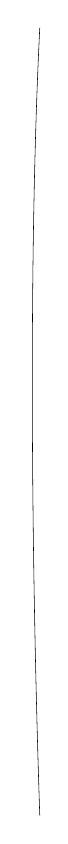
\begin{tikzpicture}[x=1cm,y=1cm]\draw[very thin] (0,0)..controls (-.15,-3) and (-.1,-7)..(0,-10);\end{tikzpicture}}}
Pour $q>0$, on se réduit comme d'habitude au cas $S,X,Y$ de type fini sur $\operatorname{Spec}\mathbb Z$. De plus, il suffit \deleted{\unsure{x}} évidemment de traiter le cas ou $S'=\overline s$ est un point \deleted{\unsure{geo}} géométrique de $S$ (cf. XII.6.5).
\margin{!}
Supposons que $F$ soit un faisceau de \deleted{groupes} ind $\mathbb L$-groupes. Si la codimension de $(Y,X)$ n'est pas 1 \deleted{\unsure{,}} (nous le supposons constant), on a $(R^qj_*)g^*=(R^qj'_*){g'}^*=0$ (3.4), d'où le résultat. Supposons que la codimension soit 1, et soit $\overline x$ un point géométrique de $X$ au dessus de $\overline s$ tel que son image soit dans $Y$. Reprenons les \deleted{\unsure{no}} notations de la démonstration de (3.5): on a
